% !TEX root = ../main.tex
% chktex-file 21
% chktex-file 46
\section{Effects of Coarsening}%
\label{sec:cons}

We have just seen how to compute a coarsened graph $G_c$ via the REC algorithm.
What remains to be answered now is how coarsening affects the performance of graph algorithms when $G_c$ is used as a proxy for the original graph $G$.
In the first step we will introduce a graph similarity measure.
Using this measure we will then put bounds on the dissimilarity of $G$ and $G_c$.
Finally we will use those bounds to analyze the influence of coarsening on the performance of the \textit{spectral clustering algorithm}.

\subsection{Restricted Spectral Similarity}%
\label{sec:cons:rss}

To compare a graph $G$ with its coarsened version $G_c$ we will use the notion of \textit{spectral similarity}.
As we have seen before, $G$ can be viewed as an operator that transforms an input signal $x \in \mathbb{R}^N$.
We described this transform in terms of the graph's Laplacian $L$,
more specifically in terms of the Laplacian's eigenbasis ${\{ u_k \}}_{1 \leq k \leq N}$ and spectrum ${\{ \lambda_k \}}_{1 \leq k \leq N}$.
Similarly the coarsened graph $G_c$ can be described in terms of its Laplacian $L_c$.
Since $L \in \mathbb{R}^{N \times N}$ and $L_c \in \mathbb{R}^{n \times n}$ act on signal spaces of different dimensionality, they cannot be compared directly however.
Instead we compare $L$ with $\widetilde{L} = C^{\top} L_c C$, the upsampled version of $L_c$.
We say $\widetilde{L}$ is an \textit{$\varepsilon$-approximation} of $L$ iff.\  $\widetilde{L}$ scales the eigenvectors $u_k$ of $L$ by a factor of roughly $\lambda_k$ in the direction of $u_k$:
\begin{wrapfigure}{r}{0.25\textwidth}
	\centering
	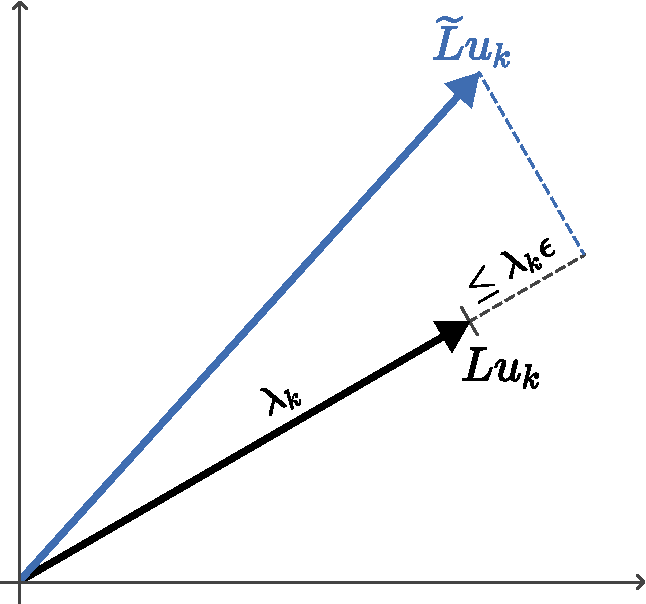
\includegraphics[width=\linewidth]{gfx/cons/rss.pdf}
	\caption{See \cref{eq:cons:rss}.}\label{fig:cons:rss}
\end{wrapfigure}
\begin{align}
	\forall k \leq K:\ (1 - \varepsilon) \underbrace{u_k^{\top} L u_k}_{\lambda_k} \leq u_k^{\top} \widetilde{L} u_k \leq (1 + \varepsilon) \underbrace{u_k^{\top} L u_k}_{\lambda_k} \text{ with } \varepsilon \geq 0\label{eq:cons:rss}
\end{align}
The reason we require \cref{eq:cons:rss} to hold only for the first $K$ eigenvectors of $L$ is, that $\text{rank}(L) = N - c$, whereas $\text{rank}(\widetilde{L}) = n - c$;
i.e.\ $\widetilde{L}$ has a higher dimensional null space\footnote{%
	Here $c$ denotes the number of connected components of $G$.
	They reduce the rank since $\lambda_1 = \cdots = \lambda_c = 0$.
}.
Thus \cref{eq:cons:rss} cannot hold for a signal $x$ that is in the null space of $\widetilde{L}$ but not in that of $L$.
Therefore the similarity condition is restricted to the first $K$ eigenvectors, as they represent the most important ``low-frequency'' components of $G$.
This restricted condition is called \textit{restricted spectral similarity} (RSS).

The choice of $K$ in RSS depends on the level of detail that should be considered when comparing $L$ and $\widetilde{L}$.
If $G$ has $c'$ clusters, i.e.\ connected subgraphs with relatively few edges going out of it, a choice of $K = c'$ is reasonable.
That way RSS checks whether the clusters of $G$ are preserved in the coarsened graph $G_c$ and how much the connectedness between the clusters changes.
Details like the connections within clusters on the other hand do not have a strong influence on the RSS similarity if $K = c'$, since they are described by the ``high-frequency'' eigenvectors $u_\ell$ of $L$ where $\ell > K$.

\subsection{Bounding REC via RSS}%
\label{sec:cons:bound}

Now we will use RSS to bound the eigenvalue distortion caused by REC coarsening.
It can be shown that the probability of satisfying the RSS condition for a single eigenvector $u_k$ with a sufficiently small eigenvalue $\lambda_k$ is lower-bounded by
\begin{align}
	\forall \lambda_k \leq \frac{\nu_\text{min}}{4}:\ P\mkern-2mu\left((1 - \varepsilon) \lambda_k \leq u_k^{\top} \widetilde{L} u_k \leq (1 + \varepsilon) \lambda_k\right)
	\geq 1 - \frac{r \nu_{\text{max}}}{2 \varepsilon d_{\text{avg}}} \left(1 + \frac{3 - 4 \lambda_k}{\nu_{\text{min}}}\right)\label{eq:cons:bound}
\end{align}
where $r = \mathbb{E}\mkern-2mu\left[\frac{N - n}{N}\right]$ is the expected graph reduction ratio, $d_{\text{avg}} = \frac{1}{N} \sum_{v_i \in \mathcal{V}} d_i$ is the average weighted vertex degree and $\nu_{\text{min}}$, $\nu_{\text{max}}$ are the minimum and maximum of the neighborhood weights ${\{ d_i + d_j - w_{i j}  \}}_{e_{i j} \in \mathcal{E}}$.
For a formal proof of this bound we refer to \citet[Suppl.~2]{Loukas2018}.
Here we will instead give an intuition for its key statements:
\begin{enumerate}[label=\textbf{\arabic*.}]
	\item \textbf{$\varepsilon$-term:}
		Unsurprisingly the RSS bound is inversely proportional to $\varepsilon$.
		Relaxing the RSS bound makes it is more likely to be satisfied.
	\item \textbf{$r$-term:}
		The RSS bound is linearly dependent on the reduction ratio $r$.
		The more the graph size is reduced, the smaller the probability of satisfying the bound.
	\item \textbf{$\lambda_k / \nu_{\text{min}}$-term:}
		There is also a linear dependence on the eigenvalue $\lambda_k$, where $\nu_{\text{min}}$ acts as a normalizing constant to make the bound independent of the scale of $\lambda_k$.
		For large eigenvalues the probability of satisfying the bound goes \textit{up}.
		This might seem counterintuitive since high-valued eigenvectors represent ``high-frequency'' components of $G$ that are more easily disturbed by coarsening than the smooth ``low-frequency'' eigenvectors.
		Thus one might expect the probability to go \textit{down} if $\lambda_k$ is large;
		and indeed this is what would happen if the RSS bound was comparing eigenvectors $u_k$ with their approximation $\widetilde{u}_k := \Pi u_k$.

		Since RSS compares $\lambda_k u_k$ with $\widetilde{L} u_k = L \widetilde{u}_k$ however, the Laplacian also has to be considered.
		When applying $L$, large eigenvalues $\lambda_k$ generally have a stronger influence on the resulting signal than small eigenvalues ${\{ \lambda_\ell \}}_{\ell \ll k}$.
		Eventhough $\langle u_\ell, \widetilde{u}_\ell \rangle > \langle u_k, \widetilde{u}_k \rangle$, $L$ weights the non-disturbed component $\langle \widetilde{u}_k, u_k \rangle u_k$ more strongly than the disturbed component $\sum_\ell \langle \widetilde{u}_k, u_\ell \rangle u_\ell$.
		As long as the eigenvector distortion is not too large ($\lambda_k \leq \frac{\nu_\text{min}}{4}$), the latter effect offsets the former, i.e.\ $\lambda_\ell \langle u_\ell, \widetilde{u}_\ell \rangle < \lambda_k \langle u_k, \widetilde{u}_k \rangle$.

		This is why large-valued eigenvectors have a larger probability of satisfying the RSS bound, up to the point where they become too large and the bound becomes undefined.
		This can be seen in \cref{fig:cons:example:regular}; it shows the RSS bound for a $20$-regular graph, which is defined up to $\lambda_{20}$, after that the eigenvector distortion becomes too large.
	\item \textbf{$\nu_{\text{max}}/d_{\text{avg}}$-term:}
		Finally the bound also depends on the quotient between the maximum weight $\nu_{\text{max}}$ within an edge neighborhood $\mathcal{N}_{i j}$ and the average weighted vertex degree $d_{\text{avg}}$.
		This quotient can be interpreted as a measure of how much the weight distribution within $G$ varies when comparing local clusters with the global average.
		Regular graphs minimize this quotient, as all their local clusters have the same weight.
		The key implication is that the distortion of the graph Laplacian caused by coarsening is proportional to the regularity of the coarsened graph, i.e.\ coarsening distorts regular graphs less than highly irregular graphs.
		This can be seen in \crefrange{fig:cons:example:regular}{fig:cons:example:bunny} for three increasingly irregular example graphs.
\end{enumerate}
\begin{figure}[ht]
	\centering
	\begin{subfigure}{0.33\textwidth}
		\includegraphics[width=\linewidth]{gfx/cons/example/regular.png}
		\caption{Regular graph ($d = 20$)}\label{fig:cons:example:regular}
	\end{subfigure}%
	\begin{subfigure}{0.33\textwidth}
		\includegraphics[width=\linewidth]{gfx/cons/example/yeast.png}
		\caption{Yeast (protein network)}\label{fig:cons:example:yeast}
	\end{subfigure}%
	\begin{subfigure}{0.33\textwidth}
		\includegraphics[width=\linewidth]{gfx/cons/example/bunny.png}
		\caption{Bunny (point cloud)}\label{fig:cons:example:bunny}
	\end{subfigure}
	\caption{%
		Comparison of the RSS-bound and the actual error constants $\varepsilon$ for the eigenvectors of multiple coarsened graphs ($r = 0.4$).
		Confidence bounds for $p_s \in \{0.5, 0.7\}$ are shown.
		\source{Loukas2018}
	}\label{fig:cons:example}
\end{figure}

\subsection{Implications for Spectral Clustering}%
\label{sec:cons:sc}
